\documentclass[10pt]{article}

%% --- Geometry / typography ---------------------------------------------------
\usepackage[margin=0.9in]{geometry}
\usepackage[T1]{fontenc}
\usepackage[utf8]{inputenc}
\usepackage{lmodern}
\usepackage{microtype}

%% --- Math / typography helpers ----------------------------------------------
\usepackage{amsmath,amssymb,amsthm}
\usepackage{bm}
\newtheorem{theorem}{Theorem}
\newtheorem{proposition}{Proposition}
\newtheorem{corollary}{Corollary}
\theoremstyle{definition}
\newtheorem{definition}{Definition}

%% --- Tables, figures, captions ----------------------------------------------
\usepackage{booktabs}
\usepackage{multirow}
\usepackage{tabularx}
\usepackage{array}
\usepackage{graphicx}
\graphicspath{{figures/}{../assets/paper1_figs/}{assets/paper1_figs/}}
\usepackage{float}
\usepackage{placeins}
\usepackage{lscape}
% TinyTeX in this environment lacks pdflscape; add the PDF rotation attribute
% that makes lscape pages open upright in standard PDF viewers.
\makeatletter
\g@addto@macro\landscape{\clearpage\pdfpageattr{/Rotate 90}}
\g@addto@macro\endlandscape{\clearpage\pdfpageattr{}}
\makeatother
\usepackage[font=small,labelfont=bf,skip=4pt]{caption}
\usepackage{subcaption}

%% --- Code listing -----------------------------------------------------------
\usepackage{xcolor}
\usepackage{listings}
\lstset{
  basicstyle=\ttfamily\footnotesize,
  breaklines=true,
  columns=fullflexible,
  keywordstyle=\color{blue!60!black}\bfseries,
  commentstyle=\color{gray}\itshape,
  stringstyle=\color{purple!50!black},
  language=Python,
  showstringspaces=false,
  numberstyle=\footnotesize\color{gray},
  frame=single, framerule=0.3pt, framesep=4pt,
  backgroundcolor=\color{gray!4},
  xleftmargin=4pt,
  literate={σ}{{$\sigma$}}1 {ρ}{{$\rho$}}1 {ε}{{$\varepsilon$}}1
}

%% --- Hyperlinks / refs ------------------------------------------------------
\usepackage[hidelinks]{hyperref}
\usepackage{url}
\usepackage{cleveref}

%% --- Misc -------------------------------------------------------------------
\usepackage{enumitem}
\setlist{nosep,leftmargin=*}
\usepackage[normalem]{ulem}
% seqsplit lets long monospace identifiers (e.g. snake_case metric names) break
% across line ends, eliminating overfull \hbox warnings on long \code{...} runs.
\usepackage{seqsplit}
% Allow extra inter-word space on the last pass to absorb the occasional
% paragraph that microtype alone cannot fit; keeps the right margin tidy
% on lines that would otherwise overflow by a few points.
\emergencystretch=3em
\setlength{\textfloatsep}{9pt plus 2pt minus 2pt}
\setlength{\floatsep}{8pt plus 2pt minus 2pt}
\setlength{\intextsep}{8pt plus 2pt minus 2pt}
\renewcommand{\floatpagefraction}{0.75}
\makeatletter
\setlength{\@fptop}{0pt}
\setlength{\@fpsep}{8pt plus 2pt}
\setlength{\@fpbot}{0pt plus 1fil}
\makeatother

%% --- Macros -----------------------------------------------------------------
% Short code-style identifiers are used only for software names or compact protocol keys.
\newcommand{\code}[1]{\texttt{\small #1}}
\newcommand{\codebrk}[1]{\texttt{\small\seqsplit{#1}}}
\newcommand{\stdmax}{\ensuremath{\sigma_{\max}}}

\ifdefined\blindsubmission
  \newcommand{\paperauthors}{Anonymous Authors}
\else
  \newcommand{\arxivauthors}{%
Guo An$^{1,*}$,
Zijing Wu$^{2,*,\ddagger}$,
Honghua Dong$^{1,*}$\\
Yuhao Yan$^{3,\ddagger}$,
Zixuan Gui$^{4,\ddagger}$,
Haochong Chen$^{4,\ddagger}$,
Xiang Wang$^{2}$\\
Yurong Ling$^{5,\dagger}$,
Qi Tian$^{5,1,\dagger}$\\[0.35em]
{\small $^{1}$Huawei Technologies Ltd.\quad
$^{2}$University of Science and Technology of China}\\
{\small $^{3}$Zhejiang University\quad
$^{4}$Tsinghua University}\\
{\small $^{5}$Guangdong Laboratory of Artificial Intelligence and Digital Economy (SZ)}\\[0.25em]
{\scriptsize Guo An: \texttt{anguo1@huawei.com}}\\[0.25em]
{\scriptsize $^{*}$Equal contribution.\quad
$^{\dagger}$Corresponding authors.}\\
{\scriptsize $^{\ddagger}$Work done during an internship at
\textit{Huawei Technologies Ltd.}.}%
}
\newcommand{\paperpubliccodeurl}{https://github.com/Anguo-star/acpc-diagnostics}
\newcommand{\arxivprimarycategory}{cs.LG}
\newcommand{\arxivcrosslistcategories}{cs.RO, eess.SY}
\newcommand{\arxivcomments}{Technical report; controlled diagnostic study; code, aggregate artifacts, and provenance manifest available in the repository}

  \newcommand{\paperauthors}{\arxivauthors}
\fi

\title{\textbf{Action-Conditioned Predictive Diagnostics\\for JEPA World Models}}
\author{\paperauthors}
\date{July 2026}
\hypersetup{
  pdftitle={Action-Conditioned Predictive Diagnostics for JEPA World Models},
  pdfkeywords={JEPA world models, predictive stability, action-conditioned diagnostics, cross-task calibration, visual corruption}
}

\begin{document}
\maketitle

\begin{abstract}
Visual changes that leave the underlying control state unchanged can still alter the futures predicted by a world model. Encoder-level invariance alone does not show whether learned dynamics amplify these changes or whether they affect planning. We study this problem with Action-Conditioned Predictive Consistency (ACPC), which rolls nominal and visually perturbed histories forward under the same action sequence and compares their predicted representations. ACPC gives exact inequalities for changes in future prediction error and squared goal cost, together with a different-state guard against trivial collapse. Across four control tasks, recorded-action eight-step ACPC reduces the error of predicting changes in eight-step latent error by $51.3\pm3.5\%$ relative to the strongest same-horizon control using zeroed or shuffled actions. Candidate-conditioned ACPC also improves prediction of planner cost changes and decision regret. Thresholds selected on source tasks reach $0.84$--$0.86$ balanced accuracy on the remaining tasks, and the resulting rule preserves useful checkpoint ordering under blur and resize without shift-specific adjustment. The same equations and evaluation procedure apply to PLDM, with thresholds selected separately for that model family.

\smallskip
\noindent\textbf{Keywords:} visual world models; predictive stability; action-conditioned diagnostics; calibration transfer; visual corruption.
\end{abstract}

\smallskip
\ifdefined\blindsubmission
\noindent\textbf{Anonymous reproducibility note:} code and data availability follow the venue's double-blind supplemental policy.
\else
\noindent\textbf{Code and data release:} \url{\paperpubliccodeurl}
\fi

%% ===========================================================================
\section{Introduction}\label{sec:intro}

World models support control by predicting the outcomes of candidate actions~\cite{hafner2025dreamerv3,hansen2024tdmpc2}. Joint-embedding predictive architectures (JEPAs) replace pixel reconstruction with prediction in representation space~\cite{lecun2022path,assran2023ijepa,bardes2024vjepa}. This can reduce pressure to model task-irrelevant visual detail~\cite{vanassel2025jointembeddingreconstruction,littwin2024jepaavoidsnoisyfeatures}, which is attractive when texture, lighting, or image quality changes without changing the control state.

Robust control, however, does not call for indiscriminate invariance. Background texture may be a nuisance, but a contact pose, doorway state, or object--goal relation must remain distinguishable when it changes the useful action. A planner also consumes predictions rather than an encoder output alone: a small encoding discrepancy can grow through learned dynamics, while a large one can contract before the cost readout. The relevant question is therefore whether the discrepancy introduced by a same-state visual perturbation remains small after the same action sequence.

Consistency must also be selective. Mapping every observation to the same point would make nominal and perturbed inputs agree perfectly while destroying information needed for action choice. A useful diagnostic must combine same-state stability with evidence that genuinely different states remain separated~\cite{gelada2019deepmdp,zhang2021dbc,bsmpc,grimm2020valueequivalence}. To inform planning, it should also indicate when predictive disagreement can change candidate costs or decisions.

We study these requirements with Action-Conditioned Predictive Consistency (ACPC). This is a diagnostic study of frozen checkpoints, not a new robust-training method. ACPC rolls a nominal history and a visually perturbed version of the same state through the predictor under a shared action sequence, measuring projected latent disagreement without a realized future or task outcome. For each pair, exact inequalities bound changes in future prediction error and, for squared-distance goals, candidate cost. A different-state margin guard rejects trivial low-radius collapse. The same predictive interface can be used across inspectable models, although numerical thresholds may remain model-family specific.

We evaluate ACPC on LeWM~\cite{maes2026lewm} under Gaussian observation noise across TwoRoom, PushT, Reacher, and Cube, and apply the same analysis to a complete PLDM sweep. When evaluated at observation noise $\sigma=0.08$, LeWM checkpoints trained without noise augmentation lose up to $74.56\pm5.55$ percentage points in planning success rate. We test whether recorded-action eight-step ACPC predicts the change in future error better than one-step ACPC and same-horizon controls with zeroed or shuffled actions. We then examine its relation to CEM candidate costs and decisions. Finally, we select thresholds on every source-task subset, evaluate them on the remaining tasks, and test the fixed Gaussian-noise rule under blur and resize.

The contributions are:
\begin{enumerate}[leftmargin=1.4em]
  \item \textbf{A target-free diagnostic of predictive sensitivity.} We define ACPC by rolling nominal and visually perturbed histories forward under the same actions. Exact bounds relate its disagreement score to future-error and goal-cost changes, while a different-state margin rules out trivial collapse.
  \item \textbf{Controlled evidence for prediction and planning relevance.} Across four tasks and training runs, recorded-action eight-step ACPC predicts visual-perturbation-induced error changes more accurately than one-step ACPC and same-horizon controls with zeroed or shuffled actions. Candidate-conditioned ACPC also adds information about CEM cost changes and decision regret.
  \item \textbf{Evaluation across tasks, visual shifts, and model families.} We evaluate every source/remaining-task partition, apply one Gaussian-noise calibration to blur and resize without shift-specific adjustment, and run the same analysis on PLDM. The procedure is shared, while numerical thresholds are selected separately for each model family.
\end{enumerate}
\section{Related Work}\label{sec:related}

Prior work relevant to ACPC falls into three groups: predictive world models, methods for visual robustness, and diagnostics of learned dynamics.

\paragraph{Predictive world models.}
World models learn dynamics for predicting the consequences of candidate actions~\cite{hafner2025dreamerv3,hansen2024tdmpc2}. JEPAs predict representations rather than pixels, as developed for images and video by I-JEPA and V-JEPA~\cite{lecun2022path,assran2023ijepa,bardes2024vjepa,assran2025vjepa2}. LeWM builds an end-to-end JEPA world model stabilized by SIGReg~\cite{maes2026lewm,eppspulley1983}; PLDM provides a different joint-embedding dynamics architecture, implemented here through \code{stable-worldmodel}~\cite{sobal2022jointembeddingpredictivearchitectures,sobal2025stresstesting,maes2026stableworldmodel}. Analyses of latent prediction explain how it can suppress nuisance or noisy features~\cite{vanassel2025jointembeddingreconstruction,littwin2024jepaavoidsnoisyfeatures,klindt2026lejepaworldmodel}, while Seq-JEPA studies the balance between invariant and equivariant prediction~\cite{ghaemi2025seqjepa}. Our focus is a frozen model: we measure how visual differences propagate through its predictor under actions.

\paragraph{Visual robustness for control.}
DrQ, DrQ-v2, and SODA improve visual control through training-time augmentation~\cite{kostrikov2020drq,yarats2022drqv2,hansen2021soda}. ViGMO and VIBR instead learn latent or value-function invariance to visual changes~\cite{vigmo,dupuis2023vibr}, while ReOI operates at test time to reduce distractor sensitivity in visual model-predictive control~\cite{chen2025reoi}. A complementary line of work uses bisimulation or value-aware objectives to preserve state distinctions that change downstream control decisions~\cite{gelada2019deepmdp,zhang2021dbc,bsmpc,grimm2020valueequivalence,voelcker2025calibratedvalueaware,toso2026bisimjepa}. ACPC does not modify training or repair observations. It evaluates a frozen checkpoint by combining same-state rollout agreement with a different-state separation guard.

\paragraph{Diagnostics of learned dynamics.}
Recent diagnostics test whether learned dynamics preserve action and temporal structure through inverse models, latent action decoding, cycle consistency, or compatibility with generated futures~\cite{chen2026atm,zhang2026deltajepa,seo2026acid,ruan2026futurecompatible,wang2026groupactions}. MWM incorporates action-conditioned consistency into training~\cite{yan2026mwm}, whereas iKCE identifies kinematic failures in long-horizon rollouts~\cite{schaefer2026kinematic}. These studies motivate examining the predictor rather than the encoder alone. ACPC complements them by comparing two visual views of the same state under shared actions and relating their rollout disagreement to the change in future prediction error.

\section{Action-Conditioned Predictive Consistency}\label{sec:acpc}

A same-state visual corruption first creates an upstream latent displacement.
For control, that displacement is only a proxy: the planner acts on predicted
futures and costs after the action-conditioned predictor has had a chance to
amplify, rotate, or contract the shift. At the same time, useful control
requires selectivity. A background perturbation should not move the predicted
future much, but an object pose, doorway state, contact state, or goal relation
that changes the useful action must remain distinguishable.

ACPC is built around this radius--margin view. The radius side asks whether two
visual views of the same underlying state remain inside a small rollout tube
under the same actions. The margin side asks whether task-different pairs stay
outside that tube. The pairwise ACPC radius gives the prediction-error and
planner-cost statements below; ATR summarizes this radius over logged anchors;
SMPR is the empirical margin guard against low-radius collapse.

\subsection{From visual perturbations to rollout tubes}\label{sec:acpc-def}

Let $h$ be a nominal observation--action history and let $\tilde h$ be a
visually perturbed view of the same underlying control state. A frozen encoder
maps them to $z=E_\theta(h)$ and $\tilde z=E_\theta(\tilde h)$. The predictor
$F_\theta$ rolls both representations forward under one shared action sequence
$\mathbf a=(a_0,\ldots,a_{H-1})$. A projection $\Pi$ selects the representation
component used by the diagnostic, and nonnegative weights $\alpha_k$ with
$\sum_{k=1}^H\alpha_k=1$ combine the $H$ future steps. Define
\begin{equation}
\bar G_{\mathbf a}(z)
=
\begin{bmatrix}
\sqrt{\alpha_1}\Pi(F_\theta^1(z,a_0));\ \cdots;\
\sqrt{\alpha_H}\Pi(F_\theta^H(z,\mathbf a))
\end{bmatrix},
\qquad
\mathrm{ACPC}_H(h,\tilde h,\mathbf a)
=
\|\bar G_{\mathbf a}(z)-\bar G_{\mathbf a}(\tilde z)\|_2 .
\label{eq:acpc-h}
\end{equation}
The map $\bar G_{\mathbf a}$ is the weighted predicted rollout. ACPC is the
distance between the clean and perturbed rollouts after the same action
intervention; it is the radius of the same-state rollout tube. This differs
from encoder shift, which is measured before actions are applied and therefore
cannot tell whether the predictor will amplify or contract the visual
displacement. Here $H$ counts future prediction steps, not history frames.
\emph{Action matched} means that both branches receive the same recorded or
candidate actions; it isolates visual sensitivity under a fixed intervention
and does not by itself certify action faithfulness. The unnormalized ACPC in
\Cref{eq:acpc-h} is the object used by the propositions. ATR below is the
normalized checkpoint-level summary used for screening.

\subsection{Common-future error drift}

The first proposition is a bookkeeping guarantee. Once two branches are
compared with the same action-matched future, their difference in prediction
error cannot exceed their rollout disagreement. The future
$Y_{\mathbf a}^H$ is not produced by either branch. It is an external target
used only for evaluation, such as the projected latent of the actually
observed future under the recorded action sequence, stacked and weighted like
$\bar G_{\mathbf a}$. If the two branches are compared with different futures,
the reverse-triangle argument no longer describes visual sensitivity.

\begin{proposition}[Common-future error-drift bound]\label{prop:target-free-error-drift}
Let $Y_{\mathbf a}^H$ be any projected external future generated from the same
state and action sequence as both prediction branches. With
\[
e_h=\|\bar G_{\mathbf a}(E_\theta(h))-Y_{\mathbf a}^H\|_2,
\qquad
e_{\tilde h}=\|\bar G_{\mathbf a}(E_\theta(\tilde h))-Y_{\mathbf a}^H\|_2,
\]
the following holds sample by sample:
\begin{equation}
|e_{\tilde h}-e_h|
\le \mathrm{ACPC}_H(h,\tilde h,\mathbf a).
\label{eq:target-free-error-drift}
\end{equation}
The adverse increase $(e_{\tilde h}-e_h)_+$ obeys the same bound. The
right-hand side can be computed without a future target at diagnostic time.
\end{proposition}
\begin{proof}
This is the reverse triangle inequality in the weighted-stacked projected-rollout space. The common action sequence is required because both errors must share the same target.
\end{proof}

The proposition bounds the difference between the two errors, not their
absolute magnitude. A small ACPC value therefore does not prove that either
prediction is accurate. It says only that, for a common action-matched future,
the visual perturbation cannot change the prediction error by more than the
paired-rollout radius. This is why the future-drift experiment predicts the
absolute change in eight-step latent error rather than claiming that low ACPC
means low prediction error.

\subsection{Planner flips as radius--margin events}

A planner flip is also a radius--margin event. A visual perturbation can
change a fixed-pool CEM decision only if it moves candidate costs enough to
cross a clean candidate gap. For LeWM's implemented goal cost, only the final
predicted representation at the candidate horizon enters the squared distance
to the goal. We therefore write
$x_j=\Pi(F_\theta^H(E_\theta(h),\mathbf a^j))$ and
$\tilde x_j=\Pi(F_\theta^H(E_\theta(\tilde h),\mathbf a^j))$ for the final
clean and perturbed endpoints of candidate $j$ in a fixed pool
$\{\mathbf a^j\}_{j=1}^K$. Their displacement is
$r_j=\|x_j-\tilde x_j\|_2$, the final-step component of ACPC. When
$\alpha_H>0$, $r_j\leq \mathrm{ACPC}_H/\sqrt{\alpha_H}$, but the planner audit
records $r_j$ directly.

\begin{proposition}[Squared goal-cost drift and fixed-pool certificates]\label{prop:exact-cost-certificate}
LeWM scores candidate $j$ against a fixed goal embedding $g$ by $C_j=\|x_j-g\|_2^2$ and $\tilde C_j=\|\tilde x_j-g\|_2^2$. Define
\begin{equation}
b_j=r_j\bigl(\|x_j-g\|_2+\|\tilde x_j-g\|_2\bigr).
\label{eq:exact-cost-bound}
\end{equation}
\emph{Candidate cost.} Every candidate satisfies $|\tilde C_j-C_j|\leq b_j$.

\emph{Decision regret.} Let $w$ and $\tilde w$ be the nominal and perturbed winners of the same pool. The clean-history decision regret satisfies
\begin{equation}
0\leq C_{\tilde w}-C_w\leq b_{\tilde w}+b_w.
\label{eq:fixed-pool-regret-bound}
\end{equation}
\emph{Winner stability.} If $w$ is unique and
\begin{equation}
\min_{j\ne w}\bigl(C_j-C_w-b_j-b_w\bigr)>0,
\label{eq:top1-certificate-main}
\end{equation}
then the perturbed branch has the same winner.

\emph{Elite-set stability.} If $\mathcal E$ is the nominal top-$k$ elite set and
\begin{equation}
\min_{i\in\mathcal E,\,j\notin\mathcal E}
\bigl(C_j-C_i-b_j-b_i\bigr)>0,
\label{eq:elite-certificate-main}
\end{equation}
the perturbed branch has exactly the same elite set.
\end{proposition}

The term $b_j$ is the most that candidate $j$'s squared goal cost can move
from the observed endpoint displacement and goal distances alone. The regret
bound says that choosing the perturbed winner on the clean branch cannot cost
more than the movement allowed for the clean and perturbed winners. The winner
and elite certificates are margin tests: after subtracting the allowed cost
movement from each clean gap, a positive remainder rules out that fixed-pool
flip. Unlike a global Lipschitz argument, \Cref{eq:exact-cost-bound} uses the
actual paired endpoints. It is worst-case tight from these quantities alone;
proofs and equality cases are in Appendix~\ref{sec:appendix-acpc-proofs}. The
certificate is not a compute-saving rule because it requires evaluating the
candidate under both matched histories.

The cross-entropy method (CEM) repeatedly fits its next proposal to the current
elite set. With common random numbers, two identical proposals generate the
same ordered candidate pool, so a certified common elite set also produces the
same next proposal.

\begin{corollary}[Conditional CEM stability]\label{cor:adaptive-cem-alignment}
Consider nominal and perturbed CEM runs initialized by the same proposal and sampled with common random numbers. While their ordered candidate pools are aligned, if \Cref{eq:elite-certificate-main} holds at the current iteration, both runs fit the same next proposal. If it holds at every iteration, the pools, proposals, and final action remain aligned by induction.
\end{corollary}

The corollary is conditional. It applies only while the two runs keep aligned
candidate pools and stops at the first iteration where the elite certificate
fails. It is a shared-pool model-cost statement, not a closed-loop return
guarantee. Appendix~\ref{sec:appendix-fixed-pool-details} specifies the
fixed-pool and adaptive-CEM evaluation contract.

\subsection{Selective consistency and semantic margins}

Small radius alone is insufficient because a constant representation would
make every same-state pair agree while erasing the distinctions a planner
needs. Selective consistency therefore couples a same-state tube with a
different-state margin. Let $\mathcal P_{\rm same}$ contain nominal/probed
histories of the same state and let $\mathcal P_{\rm diff}$ contain proxy
pairs that cross a task-relevant state distinction, such as different
positions, contact configurations, or goal relations. Let $d_\theta$ denote
their normalized rollout distance.
\begin{definition}[Selective predictive consistency]\label{def:selective-discriminability}
For radius $r$, margin $\gamma>0$, and pass probabilities
$p_{\rm same},p_{\rm diff}$, a representation is selectively consistent when
\begin{equation}
\Pr_{\mathcal P_{\rm same}}\!\left[d_\theta\le r\right]\ge p_{\rm same},
\qquad
\Pr_{\mathcal P_{\rm diff}}\!\left[d_\theta\ge r+\gamma\right]\ge p_{\rm diff}.
\label{eq:selective-discriminability}
\end{equation}
\end{definition}
The first inequality accepts same-state visual invariance only inside radius
$r$. The second inequality requires different-state proxy pairs to remain at
least $\gamma$ outside that tube. Selective Margin Pass Rate (SMPR) is the
empirical pass rate of the second inequality when $r$ is the same-state q90
tube. SMPR is designed to detect gross collapse; it does not prove semantic
validity, action faithfulness, or preservation of every task-relevant
distinction. Its role is to keep the radius diagnostic from rewarding a model
that becomes stable by making everything look the same.

\subsection{From pairwise quantities to checkpoint-level scores}\label{sec:acpc-diag}

The propositions above operate on one paired history or one fixed candidate
pool. To compare checkpoints, we convert pairwise radii into checkpoint-level
scores by normalizing each pair with a clean transition scale and summarizing
the upper tail across logged anchors. For anchor $i$, let $s_i$ be the median
norm of its clean observed transitions, including the history-to-future
boundary:
\begin{equation}
s_i=Q_{0.50}\!\left(\{\|u^{\mathrm{obs}}_{i,k}-u^{\mathrm{obs}}_{i,k-1}\|_2\}_{k=1}^{H}\right).
\label{eq:clean-transition-scale}
\end{equation}
For probe draw $m$, define the normalized radius $R^{(i,m)}$ and the checkpoint-level \emph{Action-Conditioned Trajectory Radius} (ATR):
\begin{equation}
R^{(i,m)}
=
\frac{\|\bar G_{\mathbf a_i}(E_\theta(h_i))-\bar G_{\mathbf a_i}(E_\theta(\tilde h_i^{(m)}))\|_2}
{s_i+\varepsilon},
\qquad
\mathrm{ATR}_q
=
Q_q\!\left(\left\{\frac{1}{M}\sum_{m=1}^{M}R^{(i,m)}\right\}_{i=1}^{n}\right).
\label{eq:predictive-radius}
\end{equation}
The numerator is the unnormalized ACPC radius used by the pairwise bounds. The
scale $s_i$ is an anchor-specific yardstick fixed by the clean logged
transition, not an outcome label. ATR is the high-quantile same-state tube
radius across logged anchors. We use q90 because a small number of high-radius
anchors can still create fragile planner histories; q90 is a reporting
summary, not a candidate-distribution probability and not a calibrated tail
bound.

The construction requires paired views, an inspectable encoder--predictor
path, and one common projection and normalization within a comparison. It does
not assume LeWM-specific layers, losses, or representation geometry. For model
family $\mathcal F$ and stressor $\upsilon$, thresholds $t_R$ and $t_M$ combine
the radius side and the margin-guard side into one score:
\begin{equation}
S_{\mathcal F,\upsilon}(\theta)
=
\min\!\left\{
\frac{t_R-\mathrm{ATR}_{\upsilon}(\theta)}{|t_R|+\varepsilon},
\frac{\mathrm{SMPR}_{\upsilon}(\theta)-t_M}{|t_M|+\varepsilon}
\right\}.
\label{eq:joint-diagnostic-score}
\end{equation}
The minimum makes the score selective: one failing side makes the whole score
negative. Thus $S\ge0$ means that the checkpoint passes both calibrated
conditions, $\mathrm{ATR}\le t_R$ and $\mathrm{SMPR}\ge t_M$. Computing $S$ for
a fixed checkpoint requires no task outcome, although success rates are used
when thresholds are selected on source tasks. Thresholds are learned separately
for each model family and visual-shift calibration. Given a reference
checkpoint $\theta_0$, the paired comparison is
\begin{equation}
\Delta S_{\mathcal F,\upsilon}(\theta_1;\theta_0)
=
S_{\mathcal F,\upsilon}(\theta_1)-S_{\mathcal F,\upsilon}(\theta_0)>0
\label{eq:paired-diagnostic-change}
\end{equation}
Both checkpoints use the same scoring map, so $\Delta S>0$ asks only whether
$\theta_1$ improves on $\theta_0$ under that map. The rule requires the
reference and does not imply that either checkpoint is absolutely robust.

\begin{definition}[Calibrated diagnostic region]\label{def:robust-interval}
For a fixed model family and visual-shift calibration, the diagnostic region contains checkpoints satisfying $\mathrm{ATR}\le t_R$ and $\mathrm{SMPR}\ge t_M$. Its meaning is evaluated on tasks excluded from threshold selection; raw thresholds are not assumed to transfer across model architectures.
\end{definition}

Table~\ref{tab:acpc-object-guide} summarizes the objects and where they enter
the experiments. The prediction experiment tests the common-future
error-drift proposition by asking whether recorded-action eight-step ACPC
predicts the change in eight-step latent error better than one-step ACPC or
same-horizon action-destroyed controls. The planner experiment tests the
fixed-pool and adaptive-CEM quantities. The cross-task, cross-stressor, and
PLDM analyses use the checkpoint-level ATR+SMPR score to test calibrated
threshold transfer. These are separate claims: prediction-error sensitivity,
planner relevance, and calibrated checkpoint screening are not interchangeable.

\begin{table}[H]
\centering
\caption{Reader guide to the ACPC objects.}
\label{tab:acpc-object-guide}
\footnotesize
\setlength{\tabcolsep}{4pt}
\begin{tabularx}{\linewidth}{p{0.17\linewidth}X p{0.27\linewidth}}
\toprule
Object & Intuition & Used in \\
\midrule
ACPC & Same-state rollout-tube radius under a shared action sequence. & Prediction and planner diagnostics \\
Common-future drift & How much the visual probe changes error to one action-matched future. & Future-drift experiment \\
$b_j$ & Maximum squared-cost movement allowed for candidate $j$ from its paired endpoints. & Fixed-pool planner certificates \\
ATR & q90 normalized same-state tube radius over logged anchors. & Checkpoint screening \\
SMPR & Fraction of different-state proxies that remain outside the same-state tube. & Collapse guard \\
$S$ & Worse side of the calibrated radius and margin passes. & Cross-task threshold transfer \\
$\Delta S$ & Change in $S$ relative to a reference checkpoint under the same scoring map. & Cross-stressor checkpoint ordering \\
\bottomrule
\end{tabularx}
\end{table}

\section{Experiments}\label{sec:exp}

\subsection{Evaluation setup}\label{sec:bg}

\paragraph{Models, tasks, and planning evaluation.}
LeWM~\cite{maes2026lewm} is the primary model family; PLDM~\cite{sobal2022jointembeddingpredictivearchitectures,sobal2025stresstesting} provides a second joint-embedding dynamics architecture. We evaluate TwoRoom navigation, PushT planar manipulation, Reacher arm control, and OGBench-Cube (Cube) 3D manipulation. We follow the standard LeWM latent-space MPC evaluation: CEM optimizes candidate action sequences with the frozen world model, and performance is the percentage of evaluation episodes that reach the task goal, reported as \emph{planning success rate}. The main evaluation adds Gaussian noise $\sigma=0.08$ to observations while keeping the goal image clean. Additional evaluations use Gaussian blur ($k=15$) and resize (scale $0.25$).

For each model family, the Gaussian-augmentation sweep contains a checkpoint trained without noise augmentation and checkpoints trained with full-sequence noise $\stdmax{}\in\{0.01,\ldots,0.08\}$. Each LeWM task--augmentation setting is trained with seeds 3072/3073/3074 and evaluated with seeds 42/43/44 using 100 episodes per evaluation seed. Evaluation seeds are conditional measurement replicates; the independently trained model is the replication unit. PLDM uses one independently trained model family over the same four tasks and nine augmentation levels. Its 36 checkpoints use the same evaluation seeds and episode count.

\paragraph{Diagnostic measurements.}
ATR uses 100 logged anchors, five perturbation draws, eight predicted steps, uniform horizon weights, within-anchor draw averaging, and a q90 summary across anchors. SMPR uses the same-state q90 tube, the closest-35\% different-state proxy neighborhood, and margin $0.10$. Appendix~\ref{sec:appendix-A} gives the complete normalization and threshold protocol.

\paragraph{Prediction and CEM analyses.}
To test prediction-error changes, we use 16 trajectory groups per task, four perturbation severities, and two perturbation draws. The target is the absolute change in eight-step latent prediction error between nominal and perturbed histories. A ridge model is fitted on 15 groups and evaluated on the remaining group, rotating through all 16. Every regression uses perturbation severity, encoder shift, action magnitude, and nominal dynamics. The regressions differ only in the added ACPC feature: one-step ACPC, the strongest eight-step control using zeroed or shuffled actions, or eight-step ACPC using the recorded actions.

For the CEM analysis, checkpoints trained without noise augmentation and with $\stdmax{}=0.08$ are evaluated on the same candidate pools. The reduced-budget analysis uses 100 histories per task and training run, $K=64$, top-eight elites, and eight CEM steps. The full-budget analysis uses the same 16 histories per task with the deployed $K=300$, top-30, 30-step configuration. Within each training run, ridge models are fitted on three tasks and evaluated on the fourth. We test whether candidate-conditioned five-step ACPC improves prediction of the maximum candidate-cost change, first-action RMS, and clean-history decision regret beyond perturbation severity, training condition, one-step ACPC, and the nominal top-1 margin.

\paragraph{Threshold evaluation.}
A Gaussian-sweep checkpoint meets the success-rate criterion when it attains at least 80\% of the improvement from the checkpoint trained without augmentation to the best checkpoint at evaluation noise $\sigma=0.08$, while losing no more than five percentage points on clean observations. We select $(t_R,t_M)$ on every nonempty proper subset of the four tasks and apply the thresholds unchanged to the remaining tasks. This gives 14 directional source/evaluation partitions. Metrics first average training runs within each evaluation task and then weight tasks equally; checkpoint rows are not treated as independent replicates. Success rates are used to select and evaluate thresholds, but they are not inputs to ACPC, ATR, or SMPR.

For blur and resize, each task uses the Gaussian thresholds selected on the other three tasks. We compare all 24 pairs of checkpoints trained without augmentation and with $\stdmax{}=0.08$. A pair is positive when success rate under blur or resize improves by at least five percentage points and clean success rate decreases by no more than five points. No blur- or resize-specific adjustment is made, and the transfer analysis does not rank encoder shift or one-step ACPC.

\subsection{Planning performance under observation noise}\label{sec:exp-gaussian-panel}

At evaluation noise $\sigma=0.08$, LeWM checkpoints trained without noise
augmentation lose $25.89\pm2.38$, $74.56\pm5.55$, $41.00\pm1.44$, and
$22.11\pm2.78$ percentage points in success rate on TwoRoom, PushT, Reacher,
and Cube, respectively. Gaussian augmentation improves performance over a
range of training levels whose location differs by task. Figure~\ref{fig:full-sweep-diagnostics}
compares success rate with ATR and SMPR across the complete sweep.

\begin{figure}[H]
\centering
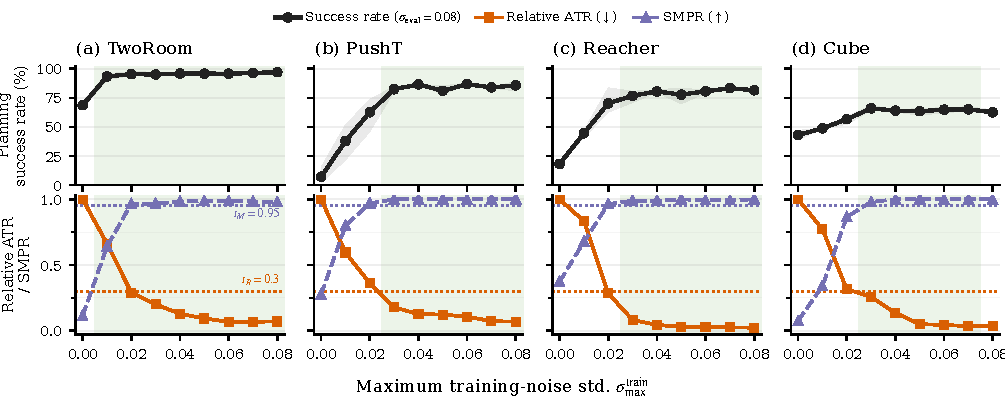
\includegraphics[width=0.95\linewidth]{fig_full_sweep_diagnostics.pdf}
\caption{Planning success rate and diagnostic measurements across the
Gaussian-augmentation sweep. Success rates use evaluation noise $\sigma=0.08$;
ATR is relative to the checkpoint trained without augmentation (value 1), and
SMPR remains on its original scale. Lines show across-run means, and shaded
ranges span the run means. Green bands mark levels that satisfy the success-rate criterion
in a majority of runs.}
\label{fig:full-sweep-diagnostics}
\end{figure}

ATR decreases and SMPR increases over the levels that meet the success-rate
criterion on every task. This association motivates the combined diagnostic,
but it does not by itself show that ACPC uses action information or predicts a
planning-relevant quantity. The next two experiments test those questions.


\subsection{Predicting error changes under visual perturbations}\label{sec:exp-target-aligned}

We first test the quantity bounded by
\Cref{prop:target-free-error-drift}:
the absolute change in eight-step latent prediction error between a nominal
history and a visually perturbed history, both compared with the same observed
future. Every regression predicts this target from the same perturbation
severity, encoder shift, action magnitude, and nominal-dynamics features. The
only difference is the ACPC feature: one-step ACPC; the better of the two
eight-step controls with zeroed or shuffled actions; or eight-step ACPC using
the recorded actions. The same-horizon comparison isolates action information
from rollout length.

\begin{figure}[H]
\centering
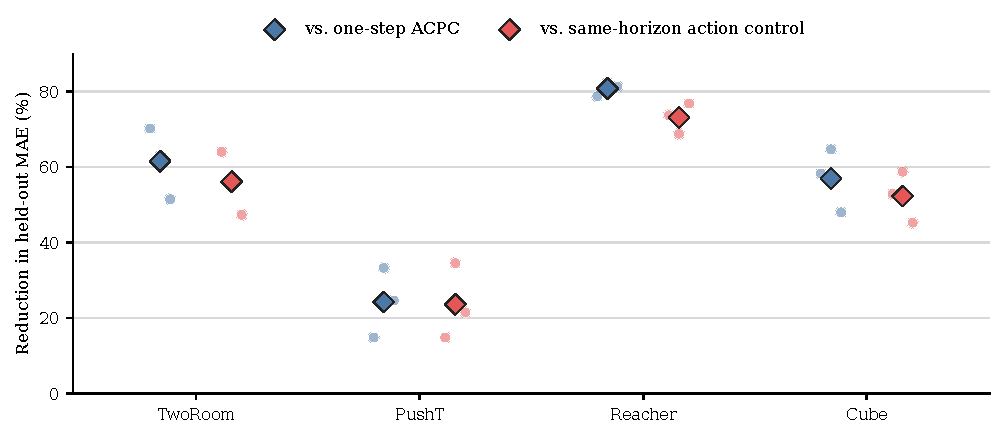
\includegraphics[width=\linewidth]{fig_future_drift_three_seed_v1.pdf}
\caption{Reduction in held-out error when recorded-action eight-step ACPC
replaces each comparator. Small circles show individual training runs and
diamonds show the mean for each task. Both comparisons predict the same
absolute change in eight-step latent prediction error. The same-horizon
control uses whichever of zeroed or shuffled actions performs better.}
\label{fig:future-drift-runs}
\end{figure}

Recorded-action eight-step ACPC reduces held-out MAE by $55.9\pm4.7\%$
relative to one-step ACPC and by $51.3\pm3.5\%$ relative to the strongest
same-horizon control (equal-task mean $\pm$ sample SD across runs). All 12
task--run comparisons improve. These results concern the ability to predict a
change in eight-step error; they do not compare the absolute accuracy of
one-step and eight-step predictions. Appendix~\ref{sec:appendix-p1-controls}
reports the task-level MAEs and selected controls.

\subsection{ACPC and CEM decisions}\label{sec:exp-planner}

We next test whether ACPC is informative about the CEM quantities in
\Cref{prop:exact-cost-certificate}. Across 9,600 reduced-budget records,
the candidate-cost bound has no violations, and the winner and elite-set
certificates never assert stability when the corresponding set changes.
Identity probes give zero five-step ACPC and zero first-action RMS. Whenever
the elite-set certificate remains valid, the nominal and perturbed CEM updates
also remain aligned, as required by Corollary~\ref{cor:adaptive-cem-alignment}.

\begin{table}[H]
\centering
\caption{Added predictive value of candidate-conditioned five-step ACPC on 9,600 reduced-budget history records. Within each training run, ridge models are fitted on three tasks and evaluated on the fourth. Both models use perturbation severity, training condition, one-step ACPC, and the nominal top-1 margin; the expanded model also uses five-step ACPC. Entries are reductions in held-out MAE, averaged equally across evaluation tasks.}
\label{tab:acpc-planner-increment}
\scriptsize
\setlength{\tabcolsep}{3.7pt}
\begin{tabular}{lrrr}
\toprule
Response & Mean $\pm$ SD & Run range & Cells improved \\
\midrule
Maximum fixed-pool cost change & 7.9 $\pm$ 1.4\% & 6.6--9.5\% & 8/12 \\
Adaptive CEM decision regret & 15.2 $\pm$ 2.0\% & 12.9--16.9\% & 12/12 \\
Adaptive first-action RMS & 1.1 $\pm$ 0.5\% & 0.8--1.7\% & 10/12 \\
\bottomrule
\end{tabular}
\end{table}


Adding candidate-conditioned five-step ACPC reduces held-out MAE for maximum
fixed-pool cost change by $7.9\pm1.4\%$; the reduction is positive on three of
the four tasks. For adaptive CEM, it reduces held-out MAE for positive decision
regret by $15.2\pm2.0\%$, with an improvement in every task--run cell. The
$1.1\pm0.5\%$ reduction for first-action RMS is too small to support an
incremental claim. In all three analyses, the rank association is higher for
five-step than for one-step ACPC in every task--run cell.

\begin{figure}[H]
\centering
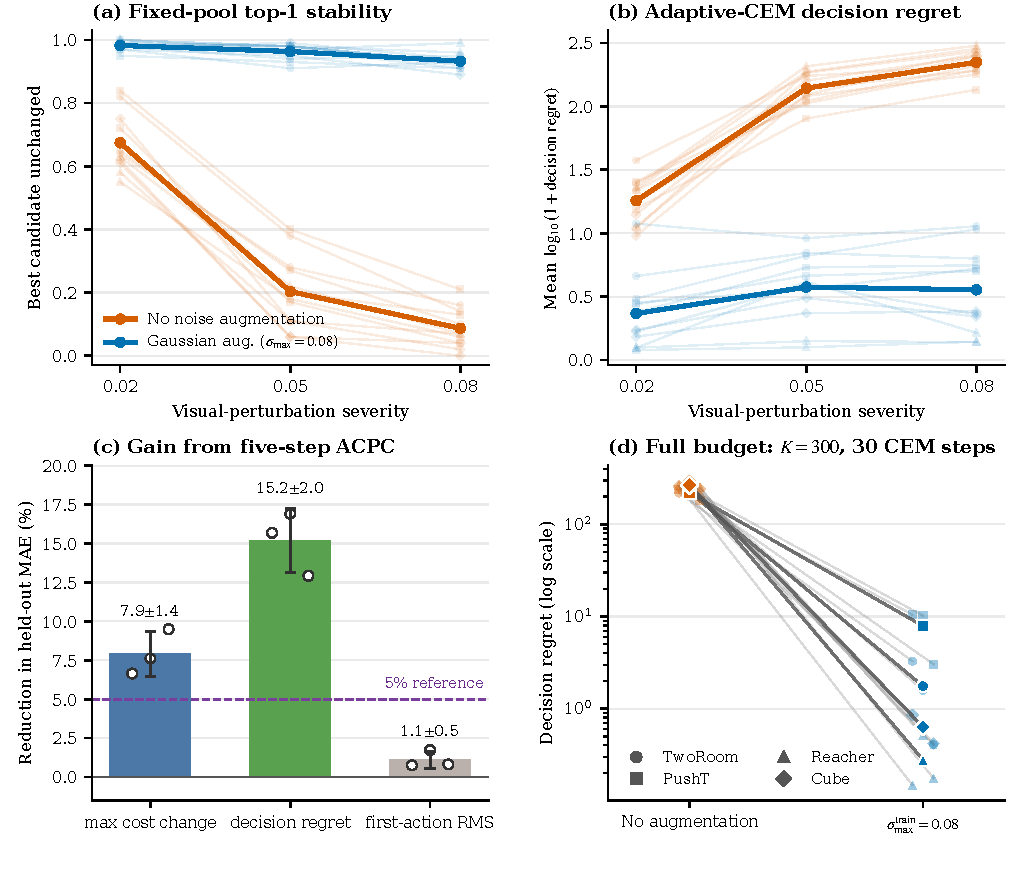
\includegraphics[width=\linewidth]{fig_acpc_planner_evidence.pdf}
\caption{ACPC and CEM decision statistics. Panels (a)--(c) use 100 histories
per task, run, and training condition: (a) best-candidate retention in a shared
pool, (b) extra clean-history latent goal cost of the perturbed CEM decision,
and (c) held-out MAE reduction from adding five-step ACPC. Panel (d) reports
decision regret on 16 shared histories per task at the deployed $K=300$,
30-step budget. Faint marks show task--run cells, heavy marks show equal-task
summaries, and error bars are sample SD across runs. Decision regret is a model
cost, not task success.}
\label{fig:acpc-planner-evidence}
\end{figure}

At perturbation severity 0.08, the task-level mean rate of retaining the best
fixed-pool candidate is $0.92$--$0.96$ after training with Gaussian
augmentation, compared with $0.02$--$0.13$ without augmentation. Mean positive
decision regret is also lower with augmentation in every task--run cell:
$3.64\pm0.68$ versus $227.04\pm16.92$ at reduced budget and $2.65\pm1.43$
versus $244.89\pm27.08$ at full budget (equal-task mean $\pm$ sample SD across
runs). Because latent cost scales differ by task, these contrasts are reported
descriptively rather than pooled as one effect. Appendix~\ref{sec:appendix-fixed-pool-details}
gives the task-level values.


\subsection{Cross-task threshold transfer}\label{sec:exp-frozen-external}

We select ATR and SMPR thresholds on every nonempty proper subset of the four
tasks and evaluate them on all remaining tasks. This gives 14 directional
partitions (Fig.~\ref{fig:cross-task-source-coverage}).

\begin{figure}[H]
\centering
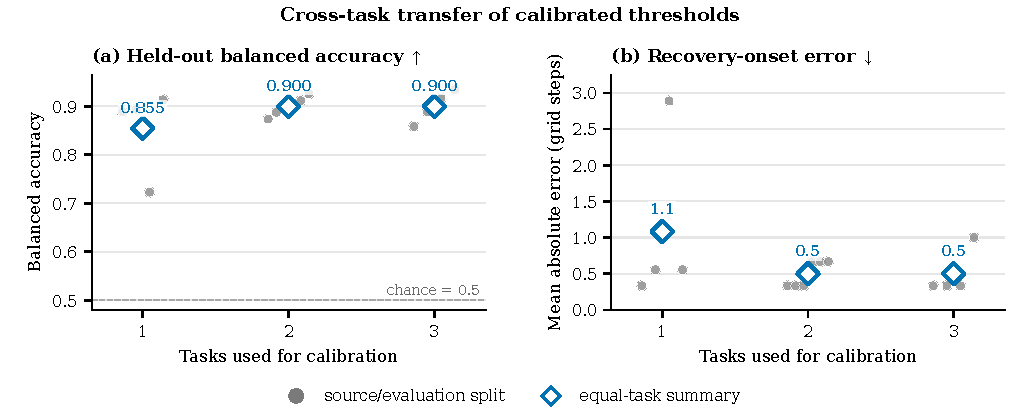
\includegraphics[width=\linewidth]{fig_cross_task_atr_smpr_source_coverage_v1.pdf}
\caption{Cross-task evaluation over all 14 source/evaluation partitions. ATR
and SMPR thresholds are selected using only the source tasks and applied
unchanged to the remaining tasks. Small points show individual partitions and
diamonds show the equal-task mean for each number of source tasks. Onset error
is the absolute difference between the first augmentation level selected by
the diagnostic and by the success-rate criterion.}
\label{fig:cross-task-source-coverage}
\end{figure}

Balanced accuracy is $0.840$, $0.855$, and $0.854$ when thresholds are
selected from one, two, and three source tasks, respectively. Corresponding
precision/recall values are $0.903/0.824$, $0.904/0.865$, and
$0.904/0.862$. Mean absolute onset errors are $0.011$, $0.010$, and $0.010$
Gaussian-augmentation-grid units, with maximum error $0.030$ at each source
coverage. Results do not improve monotonically as source tasks are added;
which tasks provide calibration data matters, particularly when TwoRoom is
held out. Thus the evaluation supports transfer of the threshold-selection
procedure across these tasks, but not one numerical threshold for every task
or model family. Appendix~\ref{sec:appendix-cross-task} reports every
partition.

\subsection{Application to PLDM}
\label{sec:exp-pldm-portability}

We apply the same paired-history construction, eight-step rollout, ATR
normalization, SMPR guard, success-rate criterion, and threshold-selection
procedure to the complete PLDM Gaussian sweep. The analysis uses PLDM's
encoder and predictor but does not depend on LeWM layers or training losses.
For each PLDM evaluation task, thresholds are selected on the other three PLDM
tasks and then fixed for its nine checkpoints.

Pooling the four evaluation branches gives $0.836$ balanced accuracy,
$0.789$ precision, and $0.882$ recall. Task balanced accuracies are $0.938$,
$0.750$, $0.500$, and $0.875$ for TwoRoom, PushT, Reacher, and Cube,
respectively; Reacher is therefore the unresolved boundary case. After
normalizing ATR within each PLDM task, applying the corresponding LeWM
source-task thresholds gives $0.807$ balanced accuracy, $0.778$ precision, and
$0.824$ recall. The shared equations and evaluation procedure therefore apply
to both LeWM and PLDM, while the raw threshold values remain model-family
specific.

\begin{table}[H]
\centering
\caption{PLDM architecture-portability check on the complete four-task, nine-checkpoint Gaussian sweep. Both rows use the current task-relative ATR score: thresholds are selected on the other three PLDM tasks or transferred from the corresponding LeWM split. Metrics pool all 36 evaluation rows. Raw numerical thresholds are not assumed to be shared across model families.}
\label{tab:pldm-architecture-portability}
\scriptsize
\setlength{\tabcolsep}{4.0pt}
\begin{tabular}{lrrrrr}
\toprule
Calibration & BA & Precision & Recall & False pass & False miss \\
\midrule
PLDM-local, other three tasks & 0.836 & 0.789 & 0.882 & 4 & 2 \\
LeWM-source reference, PLDM-anchored & 0.807 & 0.778 & 0.824 & 4 & 3 \\
\bottomrule
\end{tabular}
\end{table}


\subsection{Transfer to blur and resize}
\label{sec:exp-cross-stressor}

For each task, we apply the thresholds selected on the other three
Gaussian-noise tasks to checkpoint pairs evaluated under blur and resize. No
blur or resize result is used to select or adjust a threshold.

\begin{figure}[H]
\centering
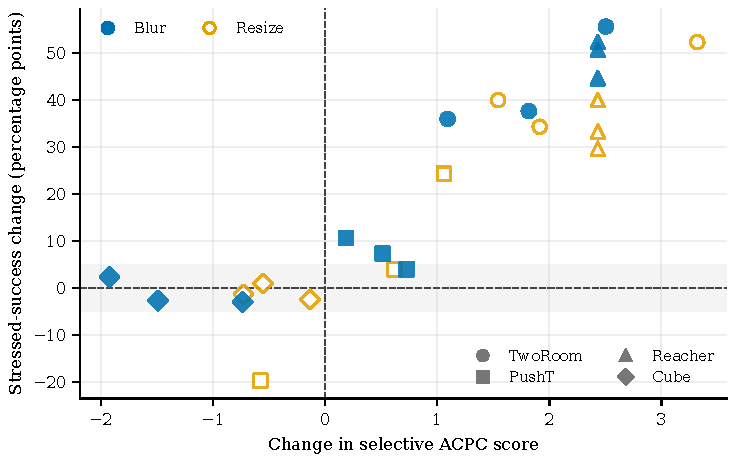
\includegraphics[width=0.92\linewidth]{fig_cross_stressor_selective_transfer_v1.pdf}
\caption{Selective-score and planning-success changes for all 24 LeWM
checkpoint pairs under blur and resize. Each point compares a checkpoint
trained with Gaussian augmentation ($\stdmax{}=0.08$) with the corresponding
checkpoint trained without augmentation. The horizontal axis uses thresholds
selected on the other three Gaussian-noise tasks; the vertical axis reports
the change in success rate under blur or resize. Marker shape denotes task and
fill denotes the visual shift.}
\label{fig:cross-stressor-selective-transfer}
\end{figure}

The sign rule reaches $0.889$ balanced accuracy, $0.882$ precision, and
$1.000$ recall, while the continuous score change has $0.909$ Spearman
correlation with the change in success rate. Blur and resize separately reach
$0.875/0.900$ balanced accuracy. The two discordant cases are both PushT
changes of exactly four percentage points, which fall below the fixed
five-point positive label while the selective score improves. These results
support relative checkpoint ordering for these two visual shifts at the tested
severity. They do not establish an absolute robustness classifier.
\FloatBarrier

\section{Discussion and limitations}\label{sec:disc}

The prediction experiment tests the quantity in
\Cref{prop:target-free-error-drift} directly. Recorded-action eight-step ACPC
predicts the change in latent error better than encoder shift, one-step ACPC,
and same-horizon controls with zeroed or shuffled actions. Because every
regression uses the same eight-step target, the result cannot be attributed
only to comparing different rollout horizons. The direction is consistent
across all tasks and runs, although the available runs do not support a precise
estimate of population-level training variability.

The CEM experiment verifies the deterministic cost bound and tests whether
candidate-conditioned ACPC explains decision changes beyond simpler features.
Its incremental gain is consistent for decision regret, positive on three of
four tasks for maximum cost change, and negligible for first-action RMS. These
are model-cost and candidate-selection results, not environment success rates.
The deployed-budget analysis also uses only 16 shared histories per task, and
the evaluation does not include matched runs without diagnostic computation;
it therefore does not estimate incremental wall-clock overhead.

Cross-task evaluation covers every source/remaining-task partition. The lack
of monotonic improvement with source-set size shows that calibration depends
on task composition. The PLDM experiment extends the equations and analysis
procedure to a second joint-embedding dynamics architecture, while confirming
that raw thresholds should remain model-family specific. Blur and resize test
a narrower form of transfer: the Gaussian-calibrated score preserves useful
relative checkpoint ordering at one severity for each visual shift.

Across the experiments, SMPR remains a gross-collapse guard rather than a
semantic proof, the cost certificates require candidate-wise paired
evaluation, and the adaptive result is conditional on pool alignment until an
elite certificate fails. Stable but incorrect predictions remain possible,
and SMPR cannot prove semantic validity. Important next steps are direct task
outcomes for ACPC-informed planner interventions, multiple severities for blur
and resize, richer different-state proxies, and additional model families with
different objectives and planner interfaces.

\section{Conclusion}\label{sec:conc}

ACPC measures how a same-state visual perturbation changes a world model's
predicted trajectory under fixed actions. Exact diagnostic inequalities relate
this change to prediction error and squared goal cost, and a different-state
margin guards against trivial collapse. Across four tasks, recorded-action
ACPC adds information beyond one-step and same-horizon action controls, relates
to CEM cost and decision changes, and supports thresholds that transfer to
held-out tasks. The same analysis applies to PLDM, and a Gaussian-calibrated
score retains useful checkpoint ordering under blur and resize. Numerical
thresholds remain model-family specific.
\bibliographystyle{plain}
\bibliography{references}

%% ===========================================================================
\FloatBarrier
\appendix
\section{Candidate-Cost and Fixed-Pool Analysis}\label{sec:appendix-acpc-proofs}

\paragraph{Proof of \Cref{prop:exact-cost-certificate}.}
For one candidate, suppress the index and factor the squared-distance
difference:
\begin{align}
|\tilde C-C|
&=\bigl|\|\tilde x-g\|_2^2-\|x-g\|_2^2\bigr| \\
&=\bigl|\langle \tilde x-x,\tilde x+x-2g\rangle\bigr| \\
&\le \|\tilde x-x\|_2\,\|\tilde x+x-2g\|_2 \\
&\le r\bigl(\|x-g\|_2+\|\tilde x-g\|_2\bigr)=b .
\end{align}
The first inequality is Cauchy--Schwarz and the second is the triangle
inequality.  Thus, for nominal winner $w$ and competitor $j$,
\[
\tilde C_j-\tilde C_w
\ge C_j-C_w-|\tilde C_j-C_j|-|\tilde C_w-C_w|
\ge C_j-C_w-b_j-b_w.
\]
For the perturbed winner $\tilde w$,
\[
C_{\tilde w}
\leq \tilde C_{\tilde w}+b_{\tilde w}
\leq \tilde C_w+b_{\tilde w}
\leq C_w+b_w+b_{\tilde w},
\]
which proves \Cref{eq:fixed-pool-regret-bound}; nonnegativity follows from the
optimality of $w$ on the nominal pool.
Positivity of \Cref{eq:top1-certificate-main} makes every perturbed competitor
strictly more costly than $w$.  The same argument for every
$i\in\mathcal E$ and $j\notin\mathcal E$ proves that
\Cref{eq:elite-certificate-main} preserves the exact elite set.  Strict
inequalities avoid relying on implementation-specific tie breaking.

\paragraph{Proof of \Cref{cor:adaptive-cem-alignment}.}
At iteration zero, the proposals are identical by assumption.  Common random
numbers therefore produce the same ordered action pool.  If the elite
certificate holds, both branches select the same action vectors as elites.
The CEM mean/variance update is a deterministic function of those vectors, so
the next proposals are identical.  Repeating this argument establishes pool
and proposal alignment by induction.  If a certificate fails, equality of the
elite sets is unknown; the induction stops and no later shared-pool statement
is made.

\paragraph{Relation to the weighted rollout radius.}
The planner bound uses the displacement at the cost readout horizon.  For the
weighted stack in \Cref{eq:acpc-h},
$\sqrt{\alpha_H}\,r_j\leq\mathrm{ACPC}_H$ whenever $\alpha_H>0$.  The formal
planner panel records $r_j$ directly, avoiding the looser
$1/\sqrt{\alpha_H}$ conversion.  This does not require a future target, but it
does require evaluating the candidate under both matched histories.

\paragraph{Sharpness without additional assumptions.}
Neither principal bound admits a uniformly smaller right-hand side from the
available quantities alone.  For a unit vector $u$, common target $Y=0$, and
two stacked predictions $au$ and $bu$ with $a,b\geq0$, the reverse-triangle
bound in \Cref{eq:target-free-error-drift} holds with equality.  Likewise,
setting $g=0$, $x=au$, and $\tilde x=bu$ makes
$|\tilde C-C|=|b-a|(a+b)=r(\|x-g\|_2+\|\tilde x-g\|_2)$.

\section{Evaluation and Diagnostic Protocol}\label{sec:appendix-A}

These details define the fixed evaluation and diagnostic protocol used by the
main tables.

LeWM is evaluated on PushT, TwoRoom, Reacher, and Cube with evaluation seeds
42/43/44 and 100 episodes per seed. The main evaluation perturbs observation
pixels with Gaussian noise at standard deviation 0.08 while keeping the goal
image clean. Checkpoints trained with noise use full-sequence input-side
Gaussian augmentation with $\stdmax{}\in\{0.01,\ldots,0.08\}$.

PLDM uses one independently trained model family and the same four-task,
nine-checkpoint Gaussian grid, evaluation seeds, trajectory count, paired
history construction, $H=8$ rollout statistic, and SMPR definition. For its
cross-task analysis, ATR is divided by its value for the corresponding PLDM
checkpoint trained without augmentation, and thresholds are selected on the
other three PLDM tasks. The evaluation task's success rates never enter
threshold selection. A second test applies the corresponding LeWM threshold
pair after this within-task PLDM normalization. Raw thresholds are not assumed
to be shared across model families.

Within each task and training run, let $B$ and $M$ be the success rates at
evaluation noise $\sigma=0.08$ for the checkpoint trained without augmentation
and the best checkpoint in the sweep. A checkpoint meets the success-rate
criterion when its noisy-observation success rate is at least $B+0.8(M-B)$ and
its clean success rate is no more than five percentage points below that of the
checkpoint trained without augmentation. The green spans in
\Cref{fig:full-sweep-diagnostics} require this criterion for a majority of
runs.

ATR is computed for each task, training run, and checkpoint from one
weighted-stacked horizon radius per anchor. The default is $H=8$ with uniform
$\alpha_k=1/H$. Each radius is divided by that anchor's q50 clean
observed-transition scale, including the transition from the last history
observation to the first future observation; multiple noise draws are first
averaged within the anchor, and q90 is then taken across anchors. For the sweep
display and within-family cross-task calibration, this checkpoint statistic is
also divided by the corresponding value without noise augmentation before
thresholds or run summaries are computed. SMPR uses programmatic
label-crossing state pairs, the q90 same-state radius, the closest-35\%
neighborhood, and normalized margin $0.10$. Across-run means and dispersions
are descriptive rather than population inference.

For cross-task evaluation, candidate thresholds are
$t_R\in\{0.05,0.075,0.10,0.15,0.20,0.30\}$ for task-relative ATR and
$t_M\in\{0.80,0.85,0.90,0.95\}$ for SMPR. Within each source-task subset, the
selection criterion lexicographically minimizes mean absolute onset error,
false-early and false-late counts, then maximizes balanced accuracy. The
selected pair is applied without modification to every evaluation task. No
evaluation-task label or blur/resize outcome enters threshold selection.

All summary figures and tables are rebuilt deterministically by the scripts documented in \codebrk{paper1/scripts/README.md}. Checkpoint-level diagnostics additionally require the released checkpoints and datasets. Machine-readable summaries record training seeds, evaluation seeds, and protocol hashes.

\begin{table}[t]
\centering
\caption{Summary of the nine-level Gaussian-augmentation sweep. ``Best'' denotes the augmentation level with the highest mean planning success rate at evaluation noise $\sigma=0.08$; Fig.~\ref{fig:full-sweep-diagnostics} shows every level. Relative ATR is divided by its value without noise augmentation and is lower-is-better; SMPR is reported on its original scale and is higher-is-better.}
\label{tab:full-sweep-compact}
\scriptsize
\setlength{\tabcolsep}{3.5pt}
\begin{tabular}{lrrrrrr}
\toprule
Task & No-aug. success (\%) & Best success (\%) & Best $\sigma_{\max}$ & Relative ATR & SMPR & Levels meeting criterion \\
\midrule
TwoRoom & 68.8 & 97.1 & 0.08 & 1.00$\to$0.07 & 0.34$\to$0.99 & 0.01--0.08 \\
PushT & 7.2 & 86.8 & 0.06 & 1.00$\to$0.10 & 0.44$\to$1.00 & 0.03--0.08 \\
Reacher & 18.2 & 83.3 & 0.07 & 1.00$\to$0.03 & 0.73$\to$0.99 & 0.03--0.08 \\
Cube & 43.1 & 66.0 & 0.03 & 1.00$\to$0.31 & 0.45$\to$0.99 & 0.03--0.07 \\
\bottomrule
\end{tabular}
\end{table}


\section{Prediction-Error Scope and Controls}\label{sec:appendix-p1-controls}

The common-future inequality in \Cref{prop:target-free-error-drift} has zero
numerical violations in every logged eight-step and candidate-conditioned
five-step task$\times$run$\times$training-condition cell. This is an
implementation invariant, not an independent statistical success count.

Logged-future prediction and candidate planning are different estimands: the
former predicts an independent action-matched observed future after common
covariates are supplied, whereas the latter compares candidates from the
actual planner pool. We do not infer one result from the other. The separate
panel in \Cref{sec:exp-planner} supplies planner-facing evidence with
same-pool, candidate-conditioned one- and five-step features.

The prediction-error analysis is restricted to checkpoints trained without
noise augmentation and to the listed visual probes. Every run improves on all
four tasks; the across-run mean and sample standard deviation summarize
repeatability rather than a precisely estimated population distribution.

\begin{table}[t]
\centering
\caption{Held-out future-drift prediction on fragile no-noise LeWM checkpoints. Entries are positive MAE reductions (\%) after adding correct-action H8 to common encoder+H1 covariates; destroyed H8 is the best action/time-destroyed variant. Seed 3074 is the fully frozen replication. Intervals resample task$\times$trajectory blocks conditional on both trained checkpoints.}
\label{tab:target-aligned-acpc}
\footnotesize
\setlength{\tabcolsep}{4pt}
\begin{tabular}{lrrrr}
\toprule
Task / aggregation & \multicolumn{2}{c}{Absolute drift} & \multicolumn{2}{c}{Adverse drift} \\
\cmidrule(lr){2-3}\cmidrule(lr){4-5}
& vs H1 & vs destroyed H8 & vs H1 & vs destroyed H8 \\
\midrule
TwoRoom & 57.5 & 52.6 & 57.3 & 52.4 \\
PushT   & 29.0 & 28.3 & 25.1 & 23.6 \\
Reacher & 81.8 & 73.6 & 81.8 & 73.6 \\
Cube    & 57.5 & 53.0 & 57.5 & 53.0 \\
\midrule
Seed 3073, equal-task mean & 60.8 & 54.8 & 60.4 & 54.4 \\
Seed 3074, equal-task mean & 51.4 & 47.7 & 49.6 & 45.7 \\
Two-seed mean [95\% CI] & 56.5 [51.1,61.2] & 51.9 [45.0,56.6] & 55.5 [50.1,60.2] & 50.6 [44.0,55.3] \\
\bottomrule
\end{tabular}
\end{table}

\begin{table}[t]
\centering
\caption{Leave-one-trajectory-group-out regression MAE for predicting the perturbation-induced difference between nominal and perturbed eight-step prediction errors on non-augmented checkpoints. Each row contains 16 trajectory groups. All models include perturbation severity, clean--perturbed encoder-history distance, and recorded-action one-step ACPC. The two eight-step columns add either the oracle action control or recorded-action eight-step ACPC. Within each task--run row, the oracle control is the lowest-MAE choice among zeroed, batch-permuted, and time-shuffled action features over the same 16 rotations. Lower is better.}
\label{tab:target-aligned-acpc-absolute}
\scriptsize
\setlength{\tabcolsep}{3.2pt}
\begin{tabular}{lrrrrlc}
\toprule
Task & seed & \shortstack{one-step\\baseline} & \shortstack{$+$ eight-step\\action control} & \shortstack{$+$ recorded-action\\eight-step ACPC} & \shortstack{selected\\control} & \shortstack{paired\\wins} \\
\midrule
TwoRoom & 3072 & 2.535 & 2.099 & \textbf{0.755} & time-shuffled actions & 15/16 \\
TwoRoom & 3073 & 2.336 & 2.015 & \textbf{0.866} & time-shuffled actions & 15/16 \\
TwoRoom & 3074 & 2.075 & 1.911 & \textbf{1.006} & batch-permuted actions & 13/16 \\
\addlinespace[1pt]
PushT & 3072 & 2.068 & 2.068 & \textbf{1.762} & time-shuffled actions & 11/16 \\
PushT & 3073 & 1.969 & 2.008 & \textbf{1.315} & zero actions & 13/16 \\
PushT & 3074 & 1.909 & 1.833 & \textbf{1.439} & zero actions & 13/16 \\
\addlinespace[1pt]
Reacher & 3072 & 1.358 & 1.097 & \textbf{0.288} & time-shuffled actions & 16/16 \\
Reacher & 3073 & 1.399 & 0.793 & \textbf{0.247} & time-shuffled actions & 16/16 \\
Reacher & 3074 & 1.409 & 1.136 & \textbf{0.263} & time-shuffled actions & 16/16 \\
\addlinespace[1pt]
Cube & 3072 & 1.171 & 1.037 & \textbf{0.489} & zero actions & 14/16 \\
Cube & 3073 & 1.416 & 1.212 & \textbf{0.500} & zero actions & 14/16 \\
Cube & 3074 & 1.061 & 1.008 & \textbf{0.552} & time-shuffled actions & 14/16 \\
\bottomrule
\end{tabular}
\end{table}


\section{Cross-Task Threshold Partitions}\label{sec:appendix-cross-task}

The 14 rows below are exhaustive: selecting one, two, or three of four tasks
as sources creates $4+6+4$ directional partitions. Each evaluation task
retains every training run and all nine checkpoints. The apparent
sample size is therefore not inflated by treating checkpoint rows as
independent observations.

\begin{table*}[t]
\centering
\caption{Cross-task evaluation of the selective ACPC rule. Thresholds are selected on the source tasks and applied unchanged to all remaining tasks. Metrics first average training runs within each evaluation task and then weight tasks equally. Onset error is measured in Gaussian-augmentation grid units.}
\label{tab:cross-task-all-subsets}
\small
\setlength{\tabcolsep}{3.5pt}
\begin{tabular}{>{\raggedright\arraybackslash}p{0.17\textwidth}>{\raggedright\arraybackslash}p{0.17\textwidth}rrrrr}
\toprule
Source tasks & Evaluation tasks & $\tau_R$ & $\tau_M$ & BA & P / R & \shortstack{Onset error\\mean / max} \\
\midrule
TwoRoom & PushT, Reacher, Cube & 0.3 & 0.95 & 0.888 & 0.884 / 0.981 & 0.003 / 0.010 \\
PushT & TwoRoom, Reacher, Cube & 0.3 & 0.95 & 0.894 & 0.902 / 0.956 & 0.006 / 0.010 \\
Reacher & TwoRoom, PushT, Cube & 0.1 & 0.95 & 0.723 & 0.906 / 0.540 & 0.029 / 0.050 \\
Cube & TwoRoom, PushT, Reacher & 0.3 & 0.95 & 0.913 & 0.950 / 0.938 & 0.006 / 0.010 \\
TwoRoom, PushT & Reacher, Cube & 0.3 & 0.95 & 0.874 & 0.853 / 1.000 & 0.003 / 0.010 \\
TwoRoom, Reacher & PushT, Cube & 0.3 & 0.95 & 0.887 & 0.873 / 0.972 & 0.003 / 0.010 \\
TwoRoom, Cube & PushT, Reacher & 0.3 & 0.95 & 0.903 & 0.925 / 0.972 & 0.003 / 0.010 \\
PushT, Reacher & TwoRoom, Cube & 0.3 & 0.95 & 0.896 & 0.901 / 0.935 & 0.007 / 0.010 \\
PushT, Cube & TwoRoom, Reacher & 0.3 & 0.95 & 0.912 & 0.952 / 0.935 & 0.007 / 0.010 \\
Reacher, Cube & TwoRoom, PushT & 0.3 & 0.95 & 0.926 & 0.972 / 0.907 & 0.007 / 0.010 \\
TwoRoom, PushT, Reacher & Cube & 0.3 & 0.95 & 0.858 & 0.802 / 1.000 & 0.003 / 0.010 \\
TwoRoom, PushT, Cube & Reacher & 0.3 & 0.95 & 0.889 & 0.905 / 1.000 & 0.003 / 0.010 \\
TwoRoom, Reacher, Cube & PushT & 0.3 & 0.95 & 0.917 & 0.944 / 0.944 & 0.003 / 0.010 \\
PushT, Reacher, Cube & TwoRoom & 0.3 & 0.95 & 0.935 & 1.000 / 0.869 & 0.010 / 0.010 \\
\bottomrule
\end{tabular}
\end{table*}


\section{Cross-Stressor Pairs and Discordant Cases}
\label{sec:appendix-cross-stressor}

\begin{table}[t]
\centering
\caption{Transfer of the Gaussian-calibrated selective score to blur and resize. For each task, thresholds are selected on the other three Gaussian-noise tasks and fixed; each pair compares the $\stdmax{}=0.08$ checkpoint with its unaugmented counterpart. ``Discordant'' counts pairs whose score-change sign disagrees with the observed success-rate label (\Cref{sec:exp-cross-stressor}).}
\label{tab:cross-stressor-selective-transfer}
\small
\setlength{\tabcolsep}{4pt}
\begin{tabular}{lrrrrr}
\toprule
Visual shift & Pairs & BA & Precision / recall & Spearman & Discordant \\
\midrule
All pairs & 24 & 0.889 & 0.882 / 1.000 & 0.835 & 2 \\
Blur & 12 & 0.875 & 0.889 / 1.000 & 0.873 & 1 \\
Resize & 12 & 0.900 & 0.875 / 1.000 & 0.746 & 1 \\
\bottomrule
\end{tabular}
\end{table}


Both discordant rows lie near the success-rate criterion: PushT run 3072 under
resize and PushT run 3074 under blur each improve success rate by four
percentage points, one point below the five-point criterion, while their
selective scores increase. The complete table shows these cases rather than
only the aggregate classification metrics.

\begin{landscape}
\input{tables/table_cross_stressor_all_pairs_v1}
\end{landscape}

\section{Local Gaussian Sensitivity as a Mechanistic Interpretation}
\label{sec:appendix-local-sensitivity}

For a small isotropic observation perturbation
$\delta x\sim\mathcal N(0,\sigma^2 I)$, first-order linearization of encoder
$E$ followed by rollout map $G$ gives
\begin{equation}
\mathbb E\!\left[\|\Delta G\|_2^2\right]
\approx \sigma^2\|J_GJ_E\|_F^2 .
\label{eq:local-gaussian-sensitivity}
\end{equation}
This explains one mechanism by which Gaussian noise training can contract
ACPC: it reduces the composed local sensitivity of the encoder--predictor
path. It is a local approximation, not a global robustness bound and not a
separate contribution.

\begin{figure}[H]
\centering
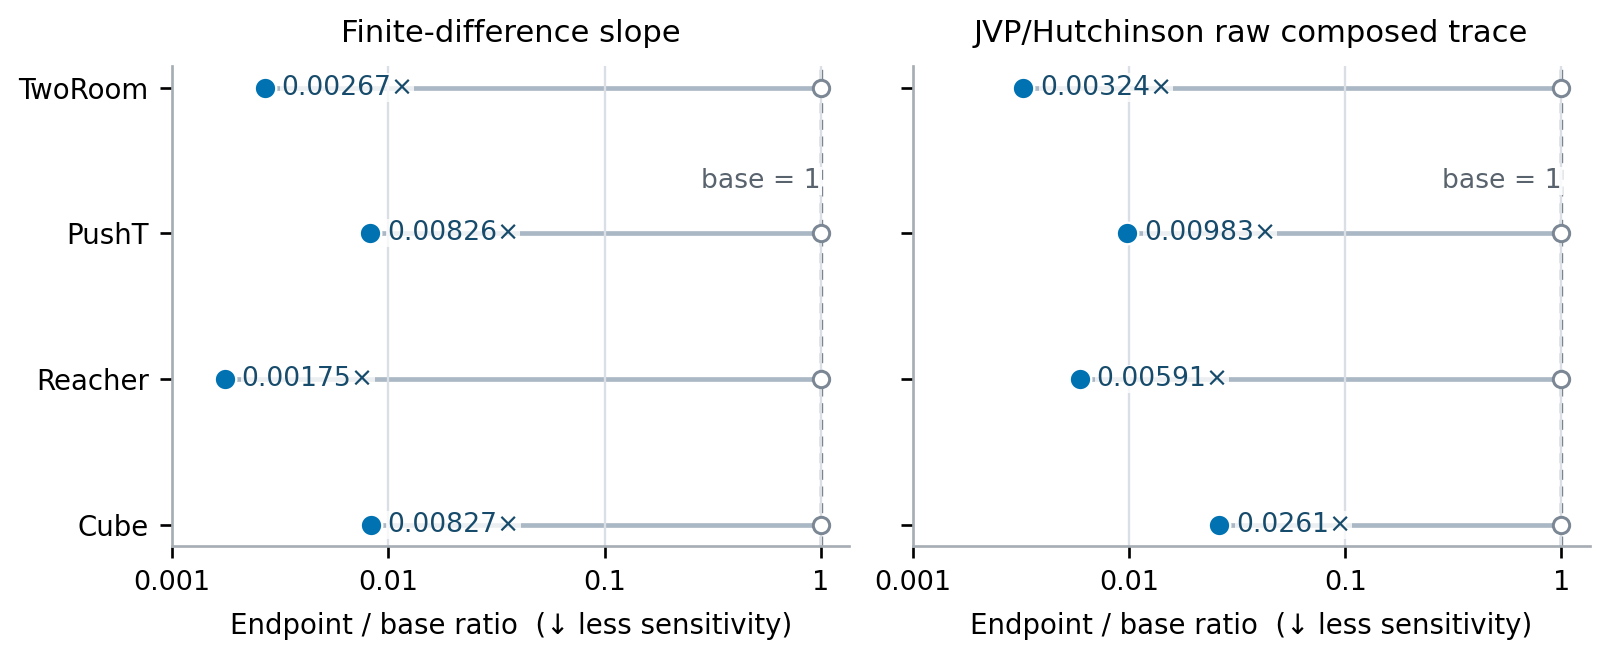
\includegraphics[width=\linewidth]{fig_gaussian_sensitivity_main.png}
\caption{Local-sensitivity ratio of the checkpoint trained with Gaussian
augmentation to the checkpoint trained without it, estimated by finite
differences and by a JVP/Hutchinson estimate of the composed Jacobian trace.
Values below one indicate contraction after augmentation. The two estimators
agree in direction for every task; these ratios do not establish task
performance.}
\label{fig:local-gaussian-sensitivity}
\end{figure}

\section{Fixed-Pool Candidate Stability}\label{sec:appendix-fixed-pool-details}

The CEM analysis does not use task-success labels. It compares checkpoints
trained without augmentation and with $\stdmax{}=0.08$ on all four tasks.
Fixed-pool shards capture the ordered initial proposal, evaluate the nominal
and perturbed histories through one shared cost path, and record exact
same-winner and elite-set events for 100 histories per task, run, and training
condition at severities $0,0.02,0.05,0.08$. Adaptive shards use a common
initial proposal and common random numbers. Proposal alignment is asserted
only while all preceding elite updates remain certified.

For nominal final plan $\mathbf a$ and perturbed plan $\tilde{\mathbf a}$, the reported positive clean-history regret is
\[
\bigl[C_h(\tilde{\mathbf a})-C_h(\mathbf a)\bigr]_+.
\]
It measures decision degradation in the model's latent goal cost, not an
environment outcome. First-action RMS is reported separately. The full-budget
evaluation keeps the same definitions but uses 16 fixed histories per task
shared across training conditions and runs, $K=300$, top-30 elites, and 30 CEM
steps. Whole-shard runtimes and forward-call counts are retained for
provenance, but without matched timing runs that omit the diagnostic they do
not estimate incremental overhead.

Across 9,600 joined reduced-budget rows there are zero
squared-distance-bound violations, zero false top-1 certificates, and zero
false elite certificates. Identity probes have zero five-step displacement
and zero first-action RMS; all identity updates remain aligned. These checks
establish implementation soundness and are not additional independent
statistical samples.

At severity $0.08$, the sufficient top-1 certificate covers $10$--$70\%$ of
histories from checkpoints trained with augmentation across task--run blocks
(and none from checkpoints trained without augmentation); elite-set coverage
is $0$--$30\%$ with augmentation. Coverage is lower than realized stability
because these conditions are sufficient but not necessary.

\begin{table}[H]
\centering
\caption{Absolute planner outcomes at Gaussian severity 0.08. Reduced-budget rows use 100 independent histories, $K=64$, top-8 elites, and eight CEM steps; full-budget rows use 16 histories, $K=300$, top-30 elites, and 30 steps. Regret evaluates the perturbed action in task-specific squared latent goal-cost units under the clean history; it is not closed-loop return, and magnitudes should not be pooled across tasks.}
\label{tab:acpc-planner-absolute}
\footnotesize
\setlength{\tabcolsep}{4.2pt}
\begin{tabular}{lrrrrrr}
\toprule
& \multicolumn{2}{c}{Top-1 stability} & \multicolumn{2}{c}{Reduced regret} & \multicolumn{2}{c}{Full-budget regret} \\
\cmidrule(lr){2-3}\cmidrule(lr){4-5}\cmidrule(lr){6-7}
Task & Base & Endpoint & Base & Endpoint & Base & Endpoint \\
\midrule
TwoRoom & 0.16 & 0.91 & 192.38 & 5.31 & 198.19 & 0.40 \\
PushT & 0.21 & 0.93 & 134.29 & 4.27 & 182.21 & 3.04 \\
Reacher & 0.07 & 0.99 & 259.89 & 0.64 & 251.95 & 0.18 \\
Cube & 0.04 & 0.89 & 248.87 & 1.20 & 242.40 & 0.42 \\
\midrule
Equal-task mean & 0.12 & 0.93 & 208.86 & 2.85 & 218.69 & 1.01 \\
\bottomrule
\end{tabular}
\end{table}


\section{Qualitative Neighborhood Visualization}\label{sec:appendix-supplementary-diagnostics}

The two-dimensional view complements the quantitative analysis by showing how repeated perturbations of the same anchors are arranged before and after noise training. Because t-SNE does not preserve metric geometry, all reported evidence remains in the original projected-rollout space.

\begin{figure}[H]
\centering
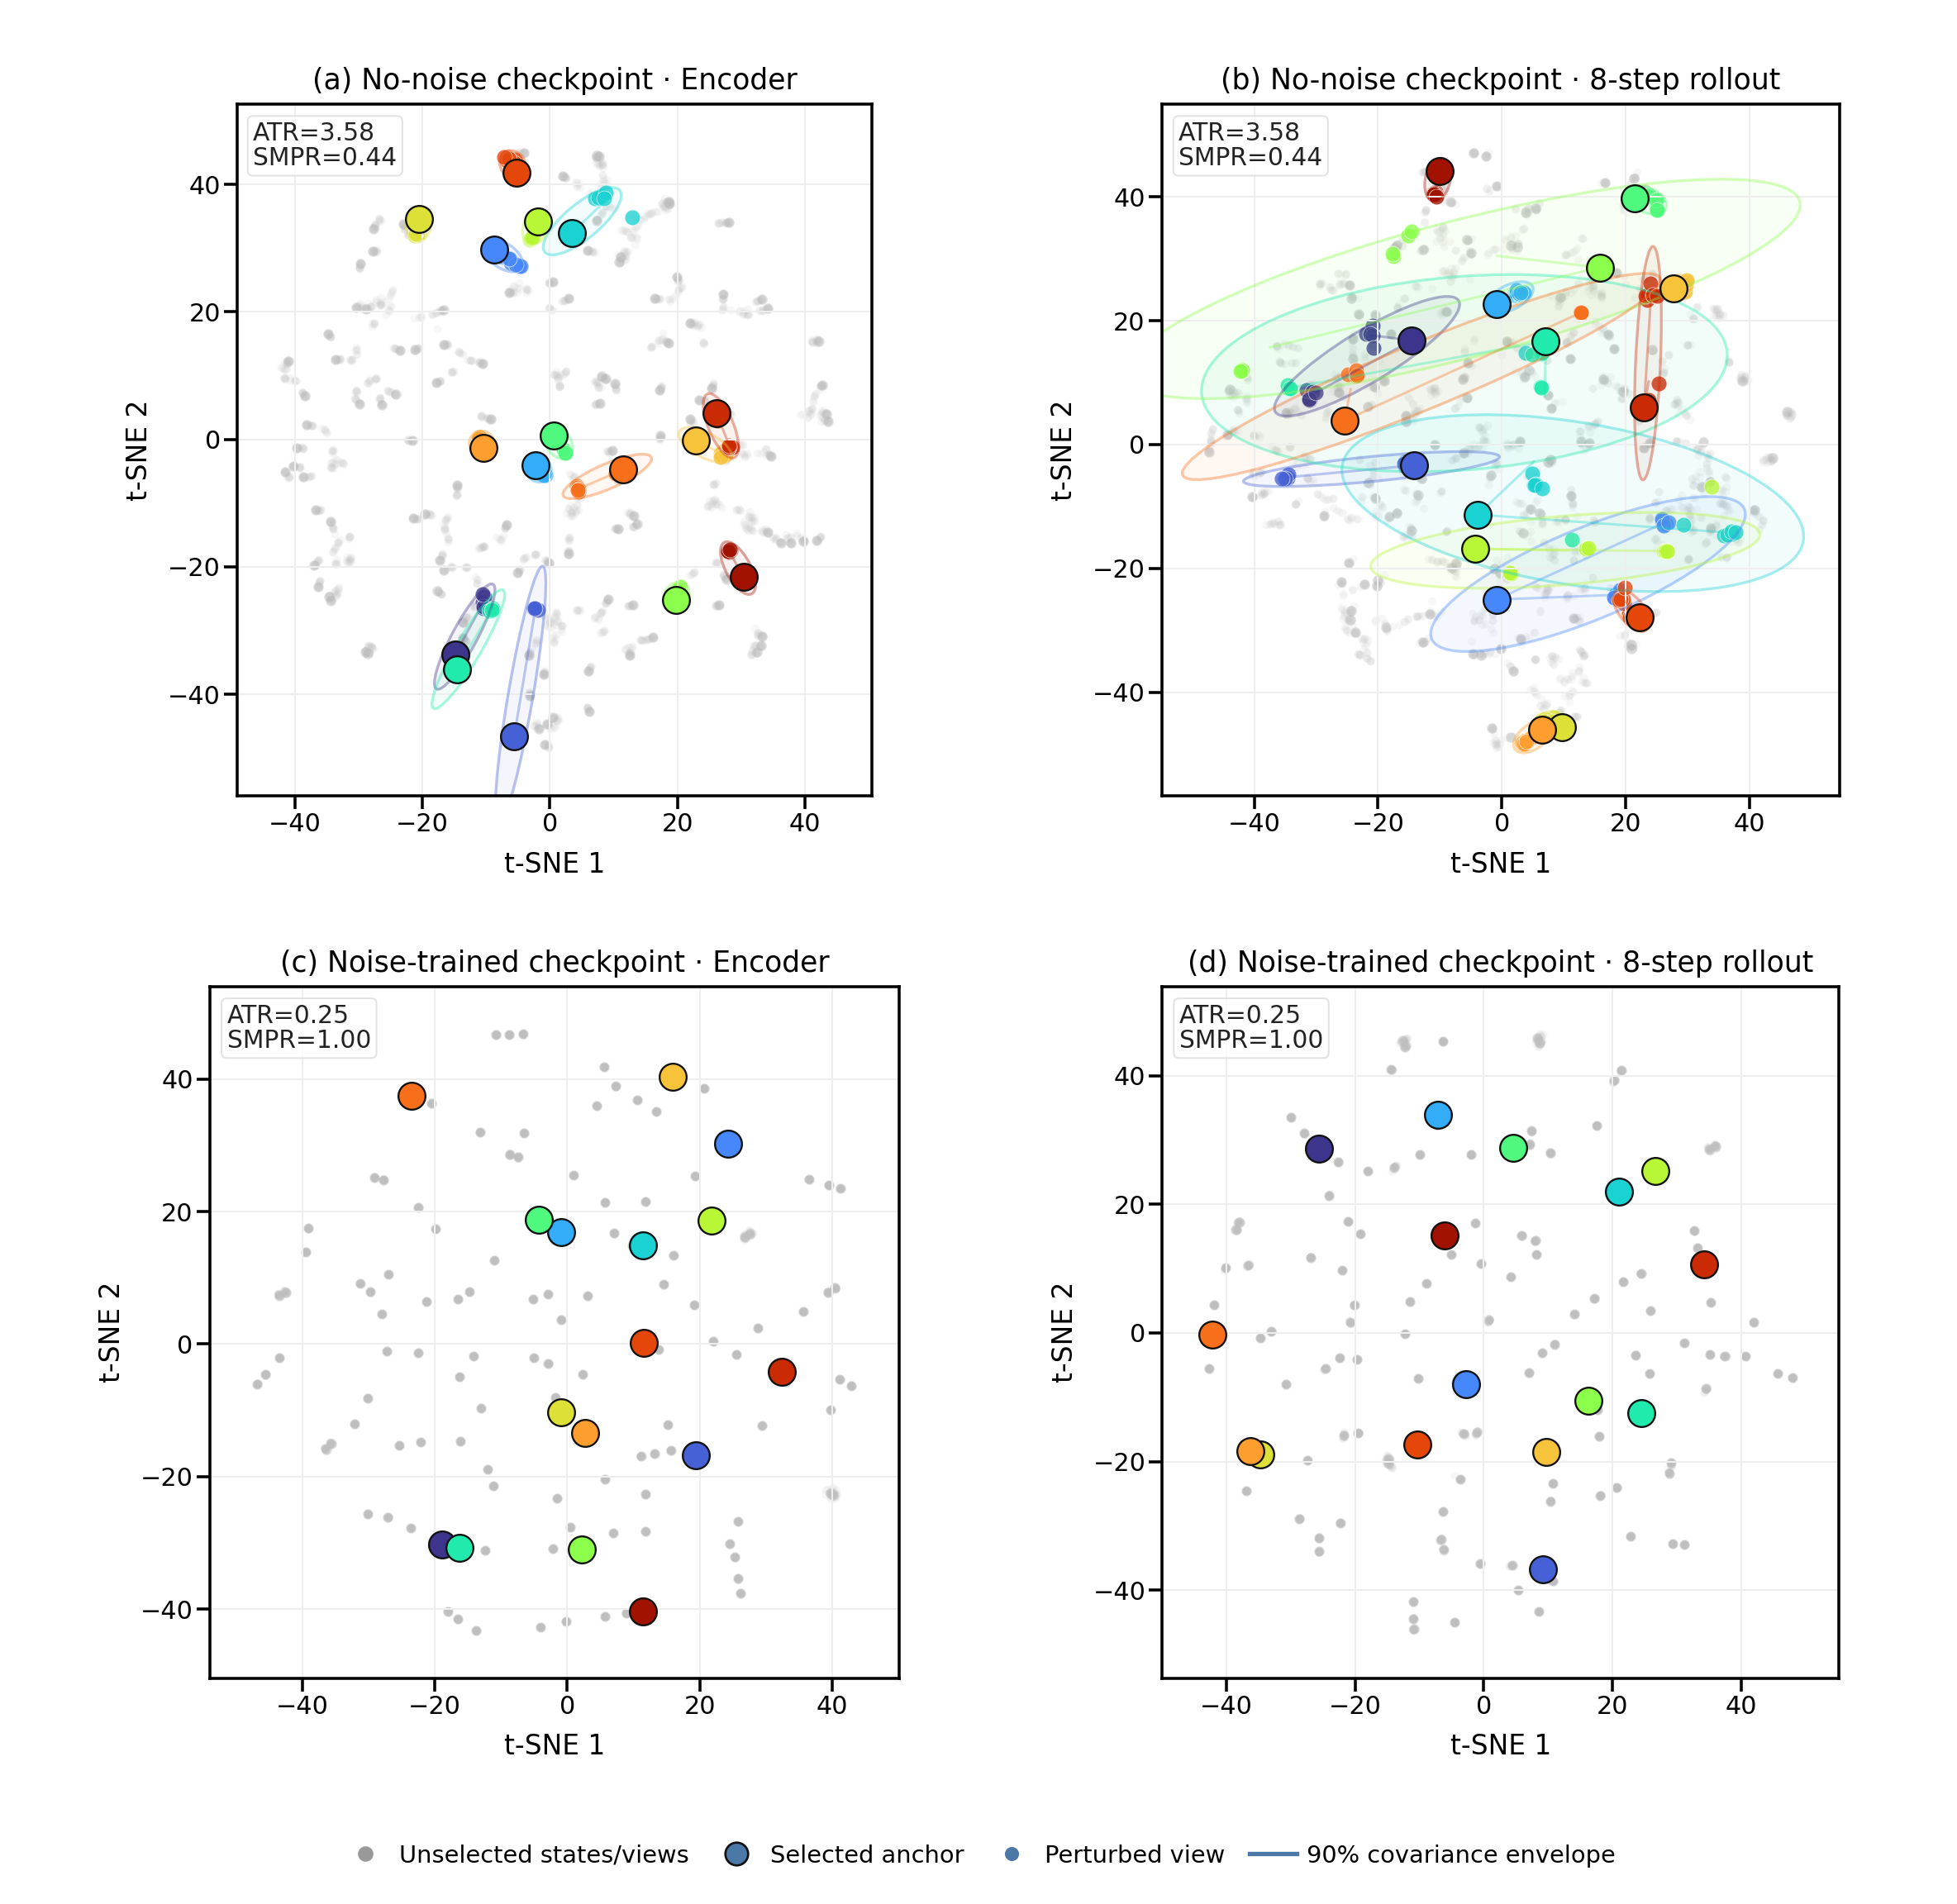
\includegraphics[width=\linewidth]{fig_acpc_basin_tsne.png}
\caption{Qualitative PushT neighborhoods for matched perturbations at
checkpoints trained without augmentation and with $\stdmax{}=0.08$, shown in
encoder and eight-step rollout spaces. t-SNE is not metric preserving: no
displayed distance, area, or overlap enters a claim; ATR and SMPR are computed
in the original space.}
\label{fig:acpc-basin-tsne}
\end{figure}

\end{document}
